\pdfoutput=1
\documentclass[11pt]{article}

% ===== Packages =====
\usepackage[utf8]{inputenc}
\usepackage[T1]{fontenc}
\usepackage{amsmath, amssymb, amsthm}
\usepackage{booktabs}
\usepackage{graphicx}
\usepackage[margin=1in]{geometry}
\usepackage[final,expansion=false]{microtype}
\usepackage[colorlinks=true, linkcolor=blue, citecolor=blue, urlcolor=blue]{hyperref}

% ===== Theorem environments =====
\theoremstyle{plain}
\newtheorem{theorem}{Theorem}
\newtheorem{lemma}[theorem]{Lemma}
\newtheorem{corollary}[theorem]{Corollary}
\theoremstyle{definition}
\newtheorem{definition}[theorem]{Definition}
\theoremstyle{remark}
\newtheorem{remark}[theorem]{Remark}

% ===== Macros =====
\newcommand{\spf}{\operatorname{spf}}
\newcommand{\Z}{\mathbb{Z}}
\newcommand{\Q}{\mathbb{Q}}
\newcommand{\C}{\mathbb{C}}
\newcommand{\re}{\operatorname{Re}}
\newcommand{\im}{\operatorname{Im}}
\DeclareMathOperator{\Li}{Li}

% ===== Title =====
\title{\textbf{The Shifted-Prime Smallest Factor Function:\\
A Computational Tour of Tension, Quadratic Splitting,\\
and the Explicit Formula}}

\author{Sadagopan Chakravarthy\thanks{
ORCID: \href{https://orcid.org/0009-0004-6166-9864}{0009-0004-6166-9864}.
Code and figures:
\url{https://github.com/s-p-c-git/PrimeSymphony}.}}

\date{June 2026}

\begin{document}
\maketitle

\begin{abstract}
For an even positive integer $k$ and odd prime $p$, define the \emph{$k$-tension}
$T_k(p) = 1/\spf(p+k)$, where $\spf$ denotes the smallest prime factor. We use
this elementary function as an organising lens for a computational tour of the
distribution of prime factors of shifted primes. We record several clean facts:
the classes $S_k(q)=\{p : \spf(p+k)=q\}$ are governed by the congruence
$p\equiv -k \pmod q$ and a quadratic-residue criterion (so the canonical case
$k=2$, $q=3$ recovers exactly the primes splitting in the Eisenstein integers
$\Z[\omega]$); the fraction of primes with $\spf(p+2)=q$ obeys an explicit
Hardy--Littlewood singular series; and isolated primes satisfy an
\emph{exactly-one-maximum} property---each carries maximal tension $1/3$ on
precisely one side, determined by $p \bmod 3$. We then exhibit the analytic
companion: the error term of the limit-orphan counting function has a Fourier
spectrum populated by the zero ordinates of both $\zeta(s)$ and $L(s,\chi_{-3})$,
and a self-contained argument-principle computation verifies that all zeros of
both functions with $|\im s|<60$ lie on the critical line. None of the
individual facts is new---the underlying mechanisms trace to Erd\H{o}s,
Hardy--Littlewood, Alladi, and a 2023 decomposition of Chavez---but their
assembly into a single elementary-to-spectral narrative, with reproducible
computation throughout, is offered as exposition.
\end{abstract}

\noindent\textbf{2020 Mathematics Subject Classification.} 11N05, 11N13, 11R11, 11M06.

\noindent\textbf{Keywords.} smallest prime factor; shifted primes; quadratic
splitting; Eisenstein integers; Dirichlet series; $L$-functions; prime zeta
function; explicit formula.

\section{Introduction}

The distribution of the prime factors of shifted values $p+k$, for $p$ prime, is
a classical subject: Erd\H{o}s showed in 1935 that $\omega(p-1)$ has normal order
$\log\log p$, and the topic remains active through the work of Pollack, Martin,
and others. In a parallel line, Alladi~\cite{Alladi1977} connected the
\emph{smallest} prime factor of integers to the prime number theorem for
arithmetic progressions, a thread extended to Chebotarev densities by
Dawsey~\cite{Dawsey2017} and others.

This note takes an elementary organising device---a ``tension'' function on
primes---and follows it from elementary number theory through to the analytic
theory of $L$-functions, recording clean facts and verifying each computationally.
We make no claim of novelty for the individual results; our aim is expository,
and we are explicit throughout about where each fact already lives in the
literature. In particular, the Dirichlet-series decomposition we use is a special
case of a general identity of Chavez~\cite{Chavez2023}, and the distributional
facts are folklore in the shifted-prime-factor community.

\paragraph{Relation to Alladi's framework.}
It is worth being precise about how the present object differs from the
Alladi--Dawsey line, since the two are easy to conflate. Alladi's identity sums
the M\"obius function $\mu(n)$ over \emph{all} integers $n$, constrained on the
smallest prime factor of $n$ \emph{itself}, and produces an exact density
identity. Here we sum over \emph{primes} $p$, constrained on the smallest prime
factor of the \emph{shifted} value $p+k$, weighted by the tension $T_k(p)$, and
produce a Dirichlet-series identity rather than a density formula. Table~1
summarises the distinction.

\begin{table}[h]
\centering
\renewcommand{\arraystretch}{1.3}
\begin{tabular}{@{}lll@{}}
\toprule
 & Alladi--Dawsey program & This note \\
\midrule
Objects & all integers $n\ge 2$ & odd primes $p$ \\
$\spf$ applied to & $n$ itself & shifted value $p+k$ \\
Weight & M\"obius function $\mu(n)$ & tension $T_k(p)=1/\spf(p+k)$ \\
Output & exact density identity & Dirichlet-series decomposition \\
\bottomrule
\end{tabular}
\caption{The present object is a shifted-prime variant of, not an instance of,
the Alladi--Dawsey framework.}
\end{table}

\paragraph{Organisation.}
Section~2 proves the classification of $S_k(q)$ via the Legendre symbol and the
resulting period law. Section~3 records the tension-fraction singular series.
Section~4 isolates the exactly-one-maximum property of isolated primes.
Section~5 turns to the analytic side: the Dirichlet decomposition, the explicit
formula and its Fourier spectrum, a self-contained zero-counting verification,
and the computational pipeline from primes to zero ordinates. Section~6 records
two open questions, and Section~7 closes with scope and limitations.

\paragraph{The device.}
For even $k>0$ and odd prime $p$, set $T_k(p) = 1/\spf(p+k)$. Since $p$ is odd and
$k$ even, $p+k$ is odd, so $\spf(p+k)\ge 3$ and $T_k(p)\le 1/3$. The primes
attaining the ceiling $1/3$ form the class $\{p : 3\mid(p+k)\}$. We call primes
$p$ with $p+2$ composite \emph{orphan} primes, and the maximal-tension orphans
\emph{limit orphans}.

\section{The Classification}

\begin{lemma}[Tension bound]\label{lem:bound}
For even $k>0$ and odd prime $p$, $T_k(p)\le 1/3$.
\end{lemma}
\begin{proof}
$p$ odd and $k$ even make $p+k$ odd, so its smallest prime factor is at least $3$.
\end{proof}

For an odd prime $q$, let $d_q$ denote the fundamental discriminant of conductor
$q$: $d_q=q$ if $q\equiv 1\pmod 4$, and $d_q=-q$ if $q\equiv 3\pmod 4$. (When
$q\equiv 3\pmod 4$ we have $-q\equiv 1\pmod 4$, so $-q$ is indeed a fundamental
discriminant, and in both cases the Kronecker symbol $(d_q/\cdot)$ is a primitive
character of conductor $q$.)

\begin{theorem}[Classification]\label{thm:class}
Let $k$ be even, $q$ an odd prime with $q\nmid k$, and $a=(-k\bmod q)$. Then
\[
S_k(q) = \{p \text{ prime}: p\equiv a \pmod q\}\setminus
\bigcup_{r<q}S_k(r),
\]
and every $p\in S_k(q)$ has the same splitting type in $\Q(\sqrt{d_q})$,
determined by the Legendre symbol $(d_q/p)=(a/q)$:
the class \emph{splits} if $(a/q)=+1$ and is \emph{inert} if $(a/q)=-1$.
\end{theorem}
\begin{proof}
$\spf(p+k)=q$ iff $q\mid(p+k)$ and no smaller prime divides $p+k$; the first
condition is $p\equiv -k\equiv a\pmod q$. Since $(d_q/\cdot)$ has conductor $q$,
the symbol $(d_q/p)$ depends only on $p\bmod q$, so equals $(d_q/a)$ for all
$p\in S_k(q)$; and $(d_q/a)=(a/q)$ by reciprocity for the discriminant $d_q$.
\end{proof}

The identity $(d_q/p)=(a/q)$ was verified computationally across all primes below
$5000$ for $q=3,5,7,11,13,17,19$ with zero exceptions.

\begin{corollary}[Period law]\label{cor:period}
For fixed prime $q$ and varying even $k$, the splitting type of $S_k(q)$ depends
only on $k\bmod 2q$. For $q=3$ this gives a period-$6$ pattern in $k$:
$k\equiv 2\pmod 6$ splits, $k\equiv 4\pmod 6$ is inert, $k\equiv 0\pmod 6$ is empty.
\end{corollary}

\begin{corollary}[Canonical case]\label{cor:eisenstein}
$S_2(3)=\{p>3 : p\equiv 1\pmod 3\}$ is exactly the set of rational primes that
split in the Eisenstein integers $\Z[\omega]$. Every such $p$ is an orphan, and no
twin prime lies in this class.
\end{corollary}

Figure~\ref{fig:grid} displays the full classification grid; the period structure
of Corollary~\ref{cor:period} is visible down each column.

\begin{figure}[t]
\centering
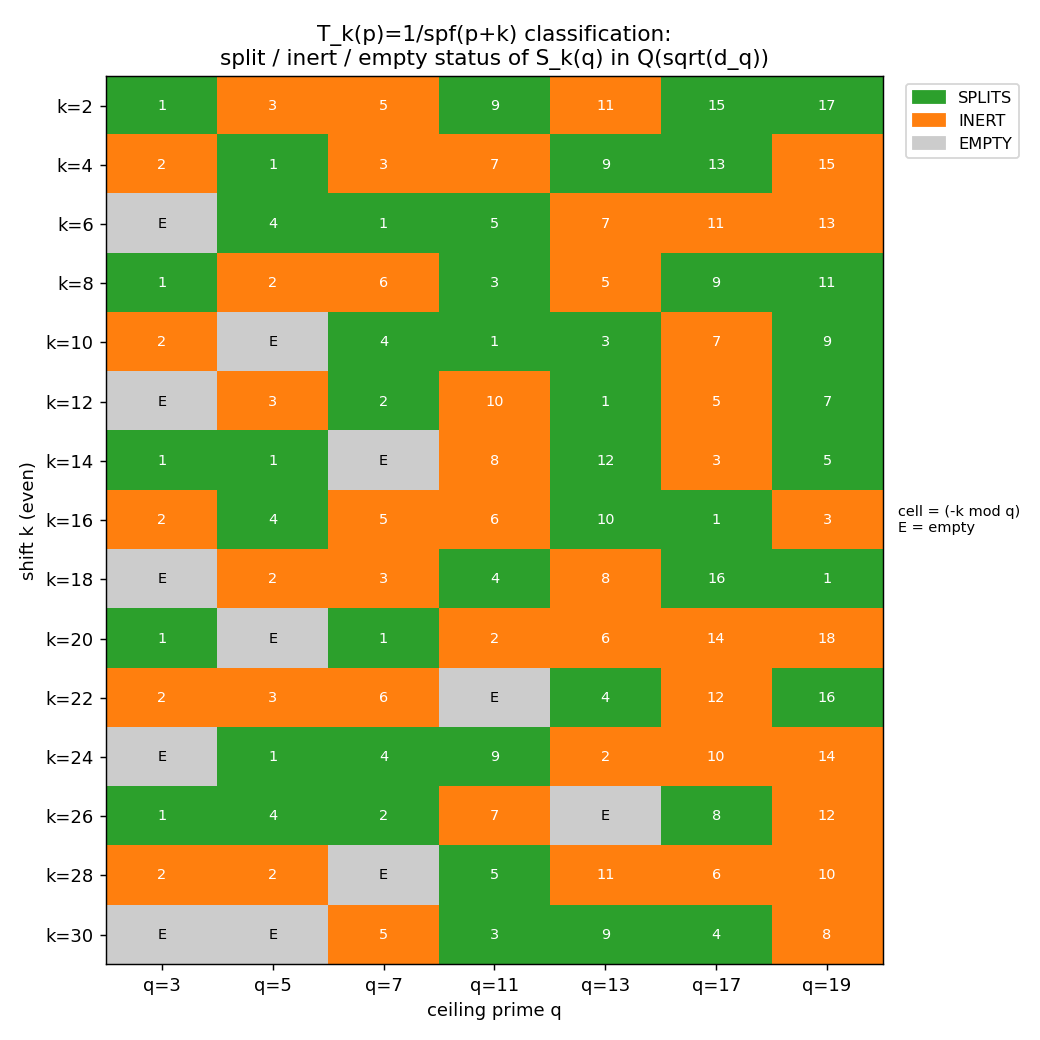
\includegraphics[width=0.78\textwidth]{figures/fig_classification_grid.png}
\caption{Splitting type of $S_k(q)$ in $\Q(\sqrt{d_q})$ for even $k$ and small
primes $q$. Each cell shows the residue $-k\bmod q$; ``E'' marks empty classes.
The $q=3$ column cycles split/inert/empty with period $6$ in $k$.}
\label{fig:grid}
\end{figure}

\section{The Tension Spectrum}

How are the tension values distributed? The following local-density law is a
Hardy--Littlewood singular series; we record it because it is clean and because
it explains the empirical deficits below the naive $1/(q-1)$.

\begin{theorem}[Tension-fraction law]\label{thm:singular}
Among primes $p$, the density of those with $\spf(p+2)=q$ is
\[
\frac{1}{q-1}\prod_{\substack{r\text{ prime}\\ 3\le r<q}}\frac{r-2}{r-1}.
\]
\end{theorem}
\begin{proof}[Sketch]
The event $q\mid(p+2)$ has density $1/(q-1)$ among primes by the prime number
theorem for arithmetic progressions. Conditionally, for each odd prime $r<q$ the
event $r\nmid(p+2)$ has local density $(r-2)/(r-1)$, and the conditions across
distinct $r$ are asymptotically independent by the Chinese Remainder Theorem, so
the densities multiply.
\end{proof}

Over the $348{,}510$ primes below $5\times10^6$ the formula matches the measured
fractions to within $1\%$ for every $q\le 41$. Summing over $q$ gives
$\approx 0.903$, which together with the measured twin fraction $0.093$ accounts
for the full mass (the small residual is the slow tail of the series).

\section{Isolated Primes: The Exactly-One-Maximum Property}

The cleanest structural fact here concerns \emph{isolated} primes---those with
both $p-2$ and $p+2$ composite. Define the two-sided tension pair
$(T(p-2),T(p+2))$.

\begin{theorem}[Exactly one maximum]\label{thm:onemax}
For every isolated prime $p>3$, exactly one of $\spf(p-2)$, $\spf(p+2)$ equals
$3$. Both-equal-$3$ and neither-equal-$3$ are impossible. Moreover the side
carrying the maximum is determined by $p\bmod 3$:
\[
p\equiv 1 \pmod 3 \iff \spf(p+2)=3 \quad(\text{right}),\qquad
p\equiv 2 \pmod 3 \iff \spf(p-2)=3 \quad(\text{left}).
\]
\end{theorem}
\begin{proof}
Every prime $p>3$ is $\equiv 1$ or $2\pmod 3$. If $p\equiv 1$, then
$p+2\equiv 0\pmod 3$ and $p+2>3$ is composite, so $\spf(p+2)=3$; while
$p-2\equiv 2\pmod 3$, so $3\nmid(p-2)$ and $\spf(p-2)\neq 3$. The case
$p\equiv 2$ is symmetric. Hence exactly one side has $\spf=3$.
\end{proof}

This gives a binary invariant---\emph{tension handedness}---on isolated primes,
tracking $p\bmod 3$ and split $50/50$ by Dirichlet's theorem. Over $283{,}586$
isolated primes below $5\times10^6$ the exactly-one-maximum property held without
exception. The non-forced (``free'') side follows the law of
Theorem~\ref{thm:singular} with the $r=3$ factor removed and renormalised to its
conditional support; this was verified to within $1.5\%$ across all $q$. The
two-sided tension sum $T(p-2)+T(p+2)$ is therefore bounded by $1/3+1/5=8/15$,
first achieved at $p=23$.

Figure~\ref{fig:joint} displays the full joint distribution of
$(\spf(p-2),\spf(p+2))$ over isolated primes: the interior of the grid is
identically zero, and the entire mass lies on the cross where one coordinate
equals $3$, with the $(3,3)$ cell itself empty---Theorem~\ref{thm:onemax} made
visible.

\begin{figure}[t]
\centering
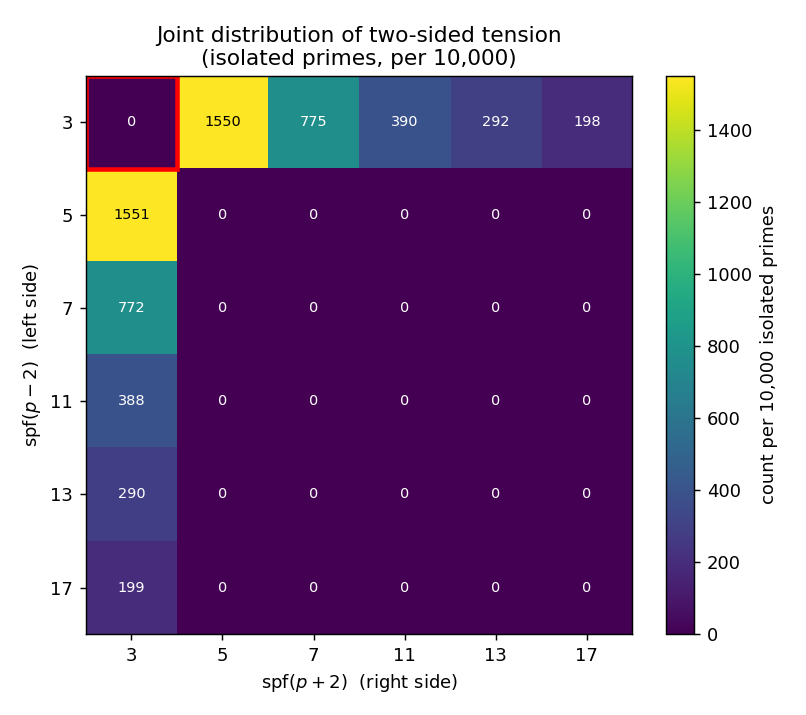
\includegraphics[width=0.62\textwidth]{figures/fig_joint_tension.png}
\caption{Joint distribution of $(\spf(p-2),\spf(p+2))$ over isolated primes.
All mass lies on the cross where one side equals $3$; the interior and the
$(3,3)$ cell (outlined) are exactly zero.}
\label{fig:joint}
\end{figure}

\section{The Analytic Companion}

We now connect the limit-orphan class to the analytic theory, recording the
duality between primes and zeros that underlies everything above.

\paragraph{Dirichlet-series decomposition.}
Writing $F_O(s)=\sum_{p\equiv 1(3)}p^{-s}$, character orthogonality mod $3$ gives
\begin{equation}\label{eq:decomp}
F_O(s) = \tfrac12\log\zeta(s) + \tfrac12\log L(s,\chi_{-3}) + G(s),
\end{equation}
where $\chi_{-3}$ is the non-principal character mod $3$ and $G(s)$ converges
absolutely for $\re(s)>1$ (with the prime-power part extending to
$\re(s)>\tfrac12$). Equation~\eqref{eq:decomp} is a special case of the general
identity of Chavez~\cite{Chavez2023}; equivalently it reflects the Dedekind
factorisation $\zeta_{\Q(\sqrt{-3})}(s)=\zeta(s)L(s,\chi_{-3})$.

\paragraph{The explicit formula and its spectrum.}
Let $\psi_O(x)=\sum_{n\le x,\,n\equiv 1(3)}\Lambda(n)$ and
$E_O(x)=\psi_O(x)-x/2$. The explicit formula for arithmetic progressions gives
\[
E_O(x) = -\tfrac12\sum_{\rho}\frac{x^\rho}{\rho}
         -\tfrac12\sum_{\rho_\chi}\frac{x^{\rho_\chi}}{\rho_\chi} + O(\log x),
\]
with $\rho$, $\rho_\chi$ the non-trivial zeros of $\zeta$ and $L(\cdot,\chi_{-3})$.
If all zeros lie on $\re(s)=\tfrac12$, then $E_O(x)/\sqrt{x}$ is a sum of cosines
in $\log x$ whose frequencies are the zero ordinates, with \emph{equal weight}
$\tfrac12$ for the two families. Computing $\psi_O(x)$ for $x\le 10^7$, taking the
Fourier transform of $E_O(x)/\sqrt{x}$, and comparing against the independently
computed zeros (Figure~\ref{fig:spectrum}) confirms this: all $15$ leading
spectral peaks match a zero of $\zeta$ or $L(\cdot,\chi_{-3})$, with the
low-lying $L$-zeros dominating because the amplitude scales as
$1/\sqrt{\gamma^2+\tfrac14}$.

\begin{figure}[t]
\centering
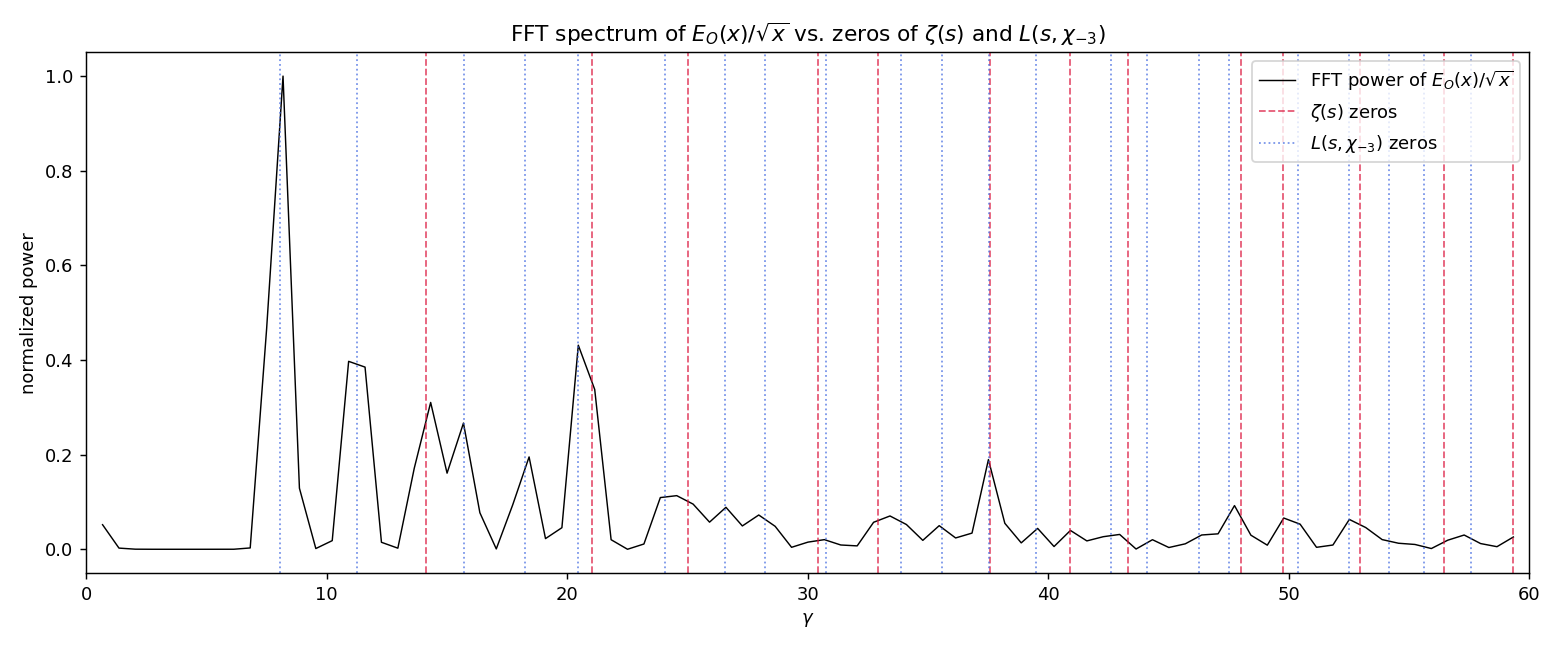
\includegraphics[width=0.92\textwidth]{figures/fig_spectrum.png}
\caption{Fourier power of $E_O(x)/\sqrt{x}$ (solid) against the zero ordinates of
$\zeta(s)$ (dashed) and $L(s,\chi_{-3})$ (dotted). Every prominent peak coincides
with a zero of one of the two functions.}
\label{fig:spectrum}
\end{figure}

\paragraph{A verified box.}
The same zeros can be \emph{counted} rigorously. Figure~\ref{fig:heatmap}
already shows where each function is small in the strip: every dark valley
sits exactly on $\re(s)=\tfrac12$. We make this rigorous via the argument
principle: for the rectangle $\Omega=\{0.1<\re s<0.9,\ |\im s|<60\}$, the
winding number around $\partial\Omega$ (evaluated to $25$ digits) gives exactly
$26$ zeros for $\zeta$ and $44$ for $L(\cdot,\chi_{-3})$, matching $2\times 13$
and $2\times 22$ on-line zeros located by sign changes (cross-checked for
$\zeta$ against the standard count). Hence every zero of both functions in
$\Omega$ is simple and on $\re(s)=\tfrac12$. This is a small-scale instance of
Turing's method; at vast scale, Platt and Trudgian~\cite{PlattTrudgian2021}
verified the Riemann hypothesis to height $3\times10^{12}$ this way.

\begin{figure}[t]
\centering
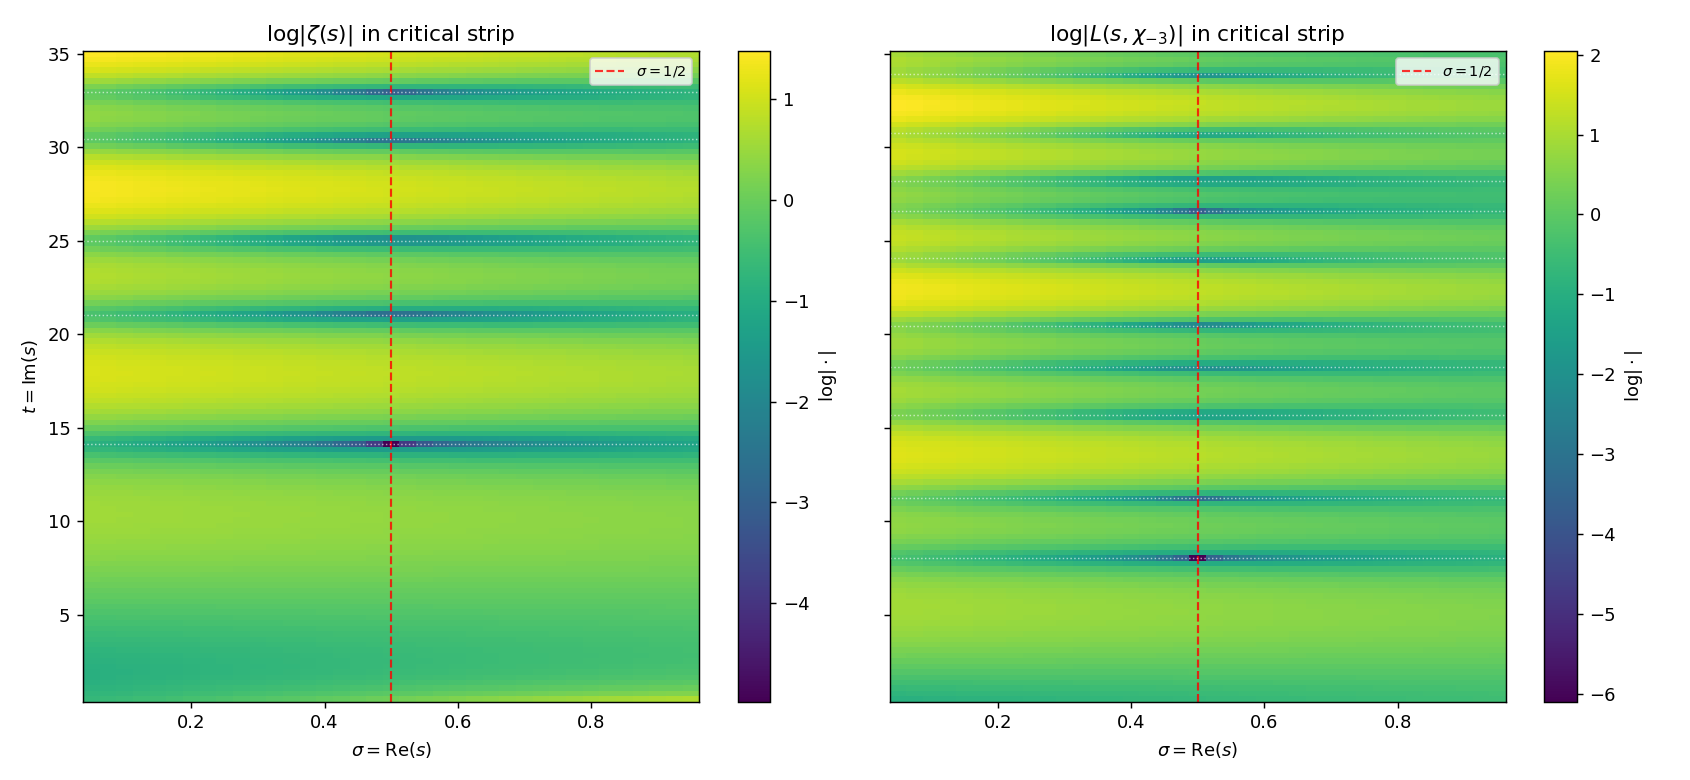
\includegraphics[width=0.97\textwidth]{figures/fig_heatmap_strip.png}
\caption{$\log|\zeta(s)|$ and $\log|L(s,\chi_{-3})|$ across the critical strip.
Every dark valley---where the function nearly vanishes---lies on
$\re(s)=\tfrac12$ (red dashed line), at heights matching the independently
located zero ordinates.}
\label{fig:heatmap}
\end{figure}

\paragraph{Primes from zeros, and a pipeline.}
The duality is genuinely two-directional in content but not in form: the zeros
reconstruct the primes as a convergent sum (sixty zeros reproduce $\psi(100)$ to
$\pm0.14$), whereas recovering the zero ordinates from prime data requires
\emph{inverting} the explicit formula. Operationally this inversion works: the
Fourier peaks of $E_O$ furnish seeds which Newton's method on the
Riemann--Siegel $Z$-function refines to machine precision in three to five steps
(Figure~\ref{fig:newton}). We note for contrast that the asymptotic seed
$\gamma_n\approx 2\pi(n-\tfrac78)/W\!\big(\tfrac{n-7/8}{e}\big)$ (Lambert $W$)
fails badly at small $n$, where its error exceeds the zero spacing; the
data-driven seeds do not. (The Lambert-$W$ seed is in fact numerically
indistinguishable from the $n$-th Gram point, to four significant figures---the
two are different routes to the same smooth approximation, and neither is a
substitute for a genuine seed near small $n$.)

\begin{figure}[t]
\centering
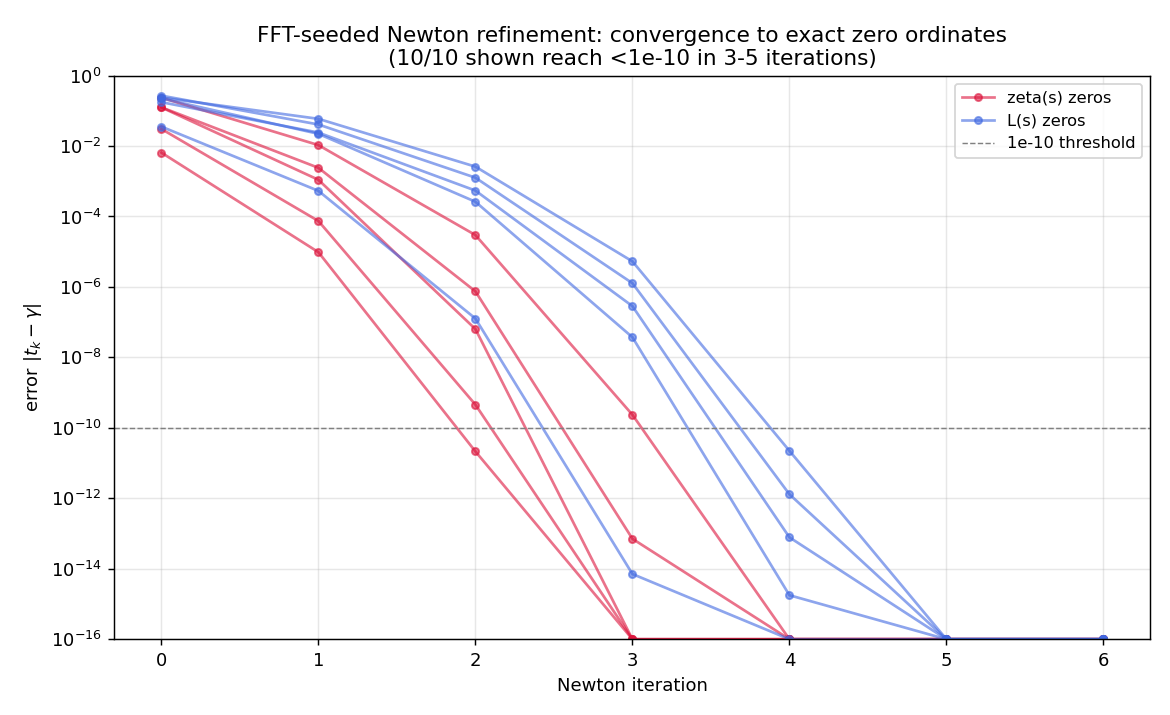
\includegraphics[width=0.82\textwidth]{figures/fig_newton_convergence.png}
\caption{Fourier-seeded Newton refinement of zero ordinates of $\zeta(s)$ and
$L(s,\chi_{-3})$. Every trace reaches machine precision within five iterations.}
\label{fig:newton}
\end{figure}

\section{Further Directions}

Two questions seem worth recording. First, the decomposition
$\zeta_{\Q(\sqrt{-3})}(s)=\zeta(s)L(s,\chi_{-3})$ raises a natural two-function
Hilbert--P\'olya question: is there a self-adjoint operator whose spectrum is
the combined ordinate set $\{\gamma_n(\zeta)\}\cup\{\gamma_n(\chi_{-3})\}$? The
most concrete single-function candidate is the Bender--Brody--M\"uller
Hamiltonian~\cite{BenderBrodyMuller2017}, whose self-adjointness remains open;
the two-function setting appears not to have been posed. A first computational
step would test whether the combined ordinate set exhibits the pair-correlation
statistics of a single random-matrix spectrum or of two superposed independent
ones. Second, the classification of Section~2 extends uniformly to other
shifts $k$ and primes $q$; whether the resulting family of Dirichlet series
admits a uniform asymptotic with an explicit error term controlled by the
relevant $L$-function zeros is, to our knowledge, unexplored.

\section{Closing Remarks}

The thread from a one-line tension bound (Lemma~\ref{lem:bound}) to a verified
statement about $L$-function zeros is short, and every step is elementary or
classical. What the device offers is organisation: it selects the Eisenstein
splitting class without invoking algebraic number theory, surfaces a clean
binary invariant on isolated primes (Theorem~\ref{thm:onemax}), and lands
naturally on the explicit formula, where the distribution of primes and the
location of zeros meet. We have been deliberate that none of this constitutes
progress on the Riemann hypothesis: the arithmetic constraints live on the real
line, while the hypothesis concerns the location of zeros in the complex plane,
and no device of this kind bridges that gap. The value, if any, is pedagogical
and computational, and the accompanying code makes every figure and number
reproducible.

\section*{Acknowledgements}
The author thanks Claude (Anthropic) for computational assistance in numerical
verification, code generation, and literature scoping. The mathematical claims
and proofs presented here reflect the author's own understanding and have been
independently reviewed by the author.

\begin{thebibliography}{9}

\bibitem{Alladi1977}
K.~Alladi,
\emph{Duality between prime factors and an application to the prime number
theorem for arithmetic progressions},
J.~Number Theory \textbf{9} (1977), 436--451.

\bibitem{BenderBrodyMuller2017}
C.~M.~Bender, D.~C.~Brody, and M.~P.~M\"uller,
\emph{Hamiltonian for the zeros of the Riemann zeta function},
Phys.\ Rev.\ Lett.\ \textbf{118} (2017), 130201.

\bibitem{Chavez2023}
G.~Chavez,
\emph{Nonlocal correlation in $L$-functions},
arXiv:2303.05611 (2023).

\bibitem{Dawsey2017}
M.~L.~Dawsey,
\emph{A new formula for Chebotarev densities},
Res.~Number Theory \textbf{3} (2017), Art.~27.

\bibitem{PlattTrudgian2021}
D.~J.~Platt and T.~S.~Trudgian,
\emph{The Riemann hypothesis is true up to $3\cdot10^{12}$},
Bull.~Lond.~Math.~Soc.~\textbf{53} (2021), no.~3, 792--797.

\bibitem{Titchmarsh}
E.~C.~Titchmarsh,
\emph{The Theory of the Riemann Zeta-Function}, 2nd ed.,
Oxford University Press, 1986.

\bibitem{Davenport}
H.~Davenport,
\emph{Multiplicative Number Theory}, 3rd ed.,
Springer, 2000.

\bibitem{IrelandRosen}
K.~Ireland and M.~Rosen,
\emph{A Classical Introduction to Modern Number Theory},
Springer, 1990.

\end{thebibliography}

\end{document}
